\section{Algorithm}%
\label{Algorithm}

\NewCryptoEntity{\Alfred}{A}
\NewCryptoEntity{\Beth}{B}
\NewCryptoEntity{\Cathy}{C}
\NewCryptoEntity{\David}{D}

We consider several participants: Alfred, Beth, Cathy and David.
Each of them has a set of devices, \(D_i\) (where \(i\in \{\Alfred, \Beth, \Cathy, 
  \David\}\)), hereafter called their device swarm.
Our system is composted of two network overlays: one protocol is run between the 
devices in \(D_i\) (the Device Swarm Protocol) to gain knowledge on the 
swarm, and another run between different swarms (the Inter-Swarm Protocol) to 
keep global knowledge.
Finally, our file-sharing protocol uses the local and global 
knowledges to coordinate file sharing between devices in different swarms.

\subsection{The Device Swarm Protocol}%
\label{DeviceSwarmProtocol}

A user's devices, \(D_i\), use the Device Swarm Protocol to coordinate 
themselves.
More specifically, the devices use this protocol to keep the swarm state up to 
date.
The swarm state contains:
\begin{itemize}
  \item A knowledge vector, \(A_i\), encoding a Markov chain to predict online 
    and offline patterns for the various devices to predict when and for how 
    long each device might be available before disappearing again;
  \item A table, \(F_i = N_i\times \powerset(D_i)\), mapping a user's file names 
    (\(N_i\)) to its devices (\(D_i\)) that store a copy of that file.
\end{itemize}

\commentDaniel{What should we reuse from the session-handoff paper?}

\subsection{The Inter-Swarm Protocol}%
\label{InterSwarmProtocol}

All swarms participate in the Inter-Swarm Protocol to coordinate the global 
knowledge needed by the swarms to interact.
More specifically, the global knowledge contains:
\begin{itemize}
  \item A table, \(R\), of devices available for routing;
  \item A key--value store, \(S = \{0, 1\}^\lambda\times \{0, 1\}^*\), mapping 
    fixed-length strings of length \(\lambda\) to arbitrary-length strings.
\end{itemize}

\subsection{File-sharing protocol}
\label{FileSharingProtocol}

\begin{figure}[t]
\centering
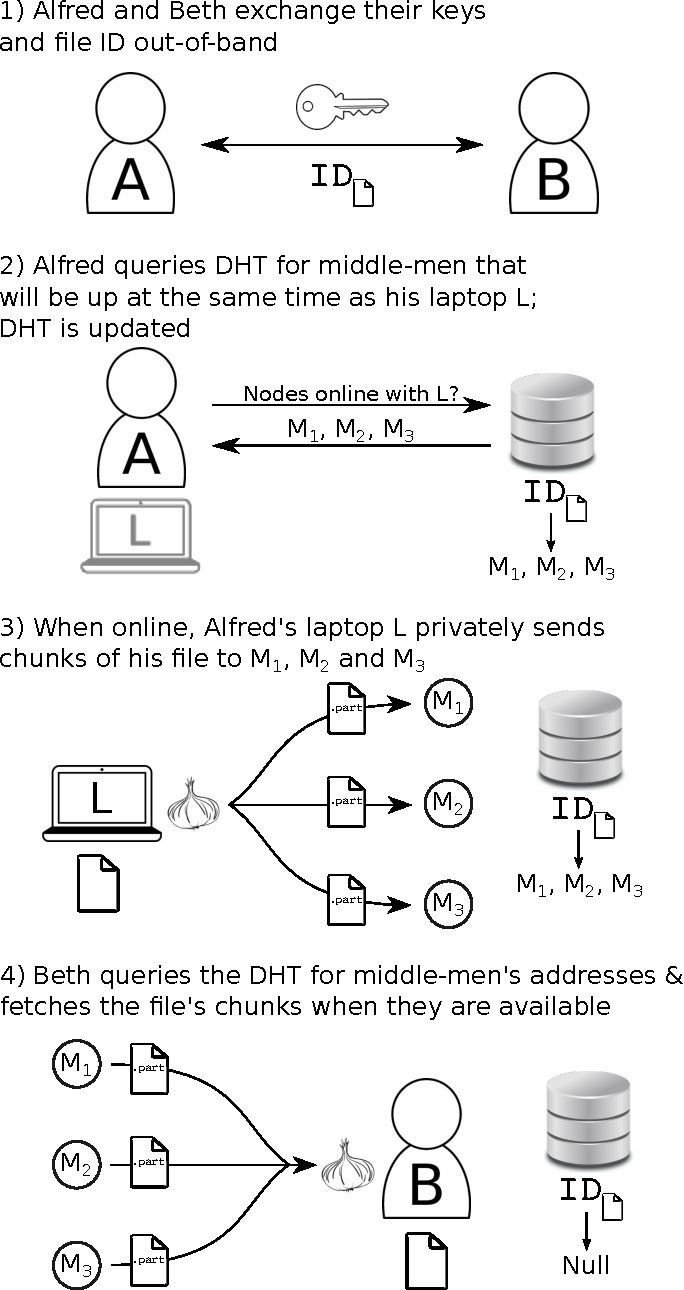
\includegraphics[width=0.8\columnwidth]{figures/schema.pdf}
\caption{\label{fig:pipeline}Pipeline of the steps undergone by Alfred when he shares a file from his laptop L with Beth.}
\end{figure}

Figure~\ref{fig:pipeline} depicts the process of a file exchange from Alfred to Beth.
The file $f$ is initially located on Alfred's laptop $L$, which is potentially offline for now.
Firstly, Alfred and Beth need to exchange encryption keys and the key $ID_f$ referencing the file on the DHT.
They do so \emph{out-of-band}, that is using another channel than the one presented here (e.g. bluetooth, email...).

Then, Alfred queries the DHT for devices that will most likely be online at the same time as his laptop $L$.
To this end, Alfred uses his knowledge on his devices connection patterns $A_i$, along with the DHT's public information on devices connections.
Once Alfred and the DHT agreed upon a set of peers $(M_1, M_2, M_3)$, their address is put in the DHT at the key $ID_f$ referencing the file of interest.

At the third step, Alfred's laptop $L$ becomes available. 
Informed of the ongoing file exchange by Alfred's Device Swarm Protocol, $L$ fetches the addresses of $M_1, M_2$ and $M_3$ on the DHT using the key $ID_f$.
These peers will serve as middle-men: $L$ sends them redundant chunks of $f$ through an onion route (thus remaining anonymous), for Beth to fetch them later.

In the last forth step, Beth fetches the file $f$ using any of her devices.
To do so, she uses the key $ID_f$ to learn the addresses of $M_1, M_2$ and $M_3$.
Then, she fetches parts of $f$ from the online middle-men through an onion route.
Given that $L$ sent redundant chunks to the middle-men, Beth will not need every middle-man to be connected to fetch the whole file.
Once Beth has completed the download, the key $ID_f$ is flushed on the DHT.

% When Alfred and Beth want to exchange a file owned by Alfred, they first need to exchange their 

% When Alfred wants to transfer a file to Beth, she will find which devices have the 
% file (from \(F_i\)), then predict when any of those devices will be available 
% (from \(A_i\)).
% Then she will construct a probabilistic onion route with her devices as the 
% destinations.
% She will encrypt this route for Beth and transfer it to him, who now can use the 
% onion route to fetch the file.